\subsection{Diseño de la base de datos}
\label{sec:diseno-bd}

El modelo relacional se implementa en SQL Server mediante \texttt{BD/esquemaBD.sql} y sus migraciones. Se separan usuarios, asignaciones, entregas y análisis confirmados mediante llaves primarias y foráneas. Los datos variables de los ejercicios y las respuestas del reconocimiento se conservan como JSON; las puntuaciones consultadas por el módulo de progreso tienen columnas numéricas.

\subsubsection{Modelo de entidades y relaciones}
La Figura~\ref{fig:er} representa el diagrama entidad relación. Un usuario tiene un perfil de tutor o alumno. Cada alumno pertenece a un tutor, y cada asignación vincula un ejercicio con el tutor que lo habilita para su grupo. El intento pertenece a un alumno y a una asignación.

\begin{landscape}
  \begin{figure}[p]
  \centering
  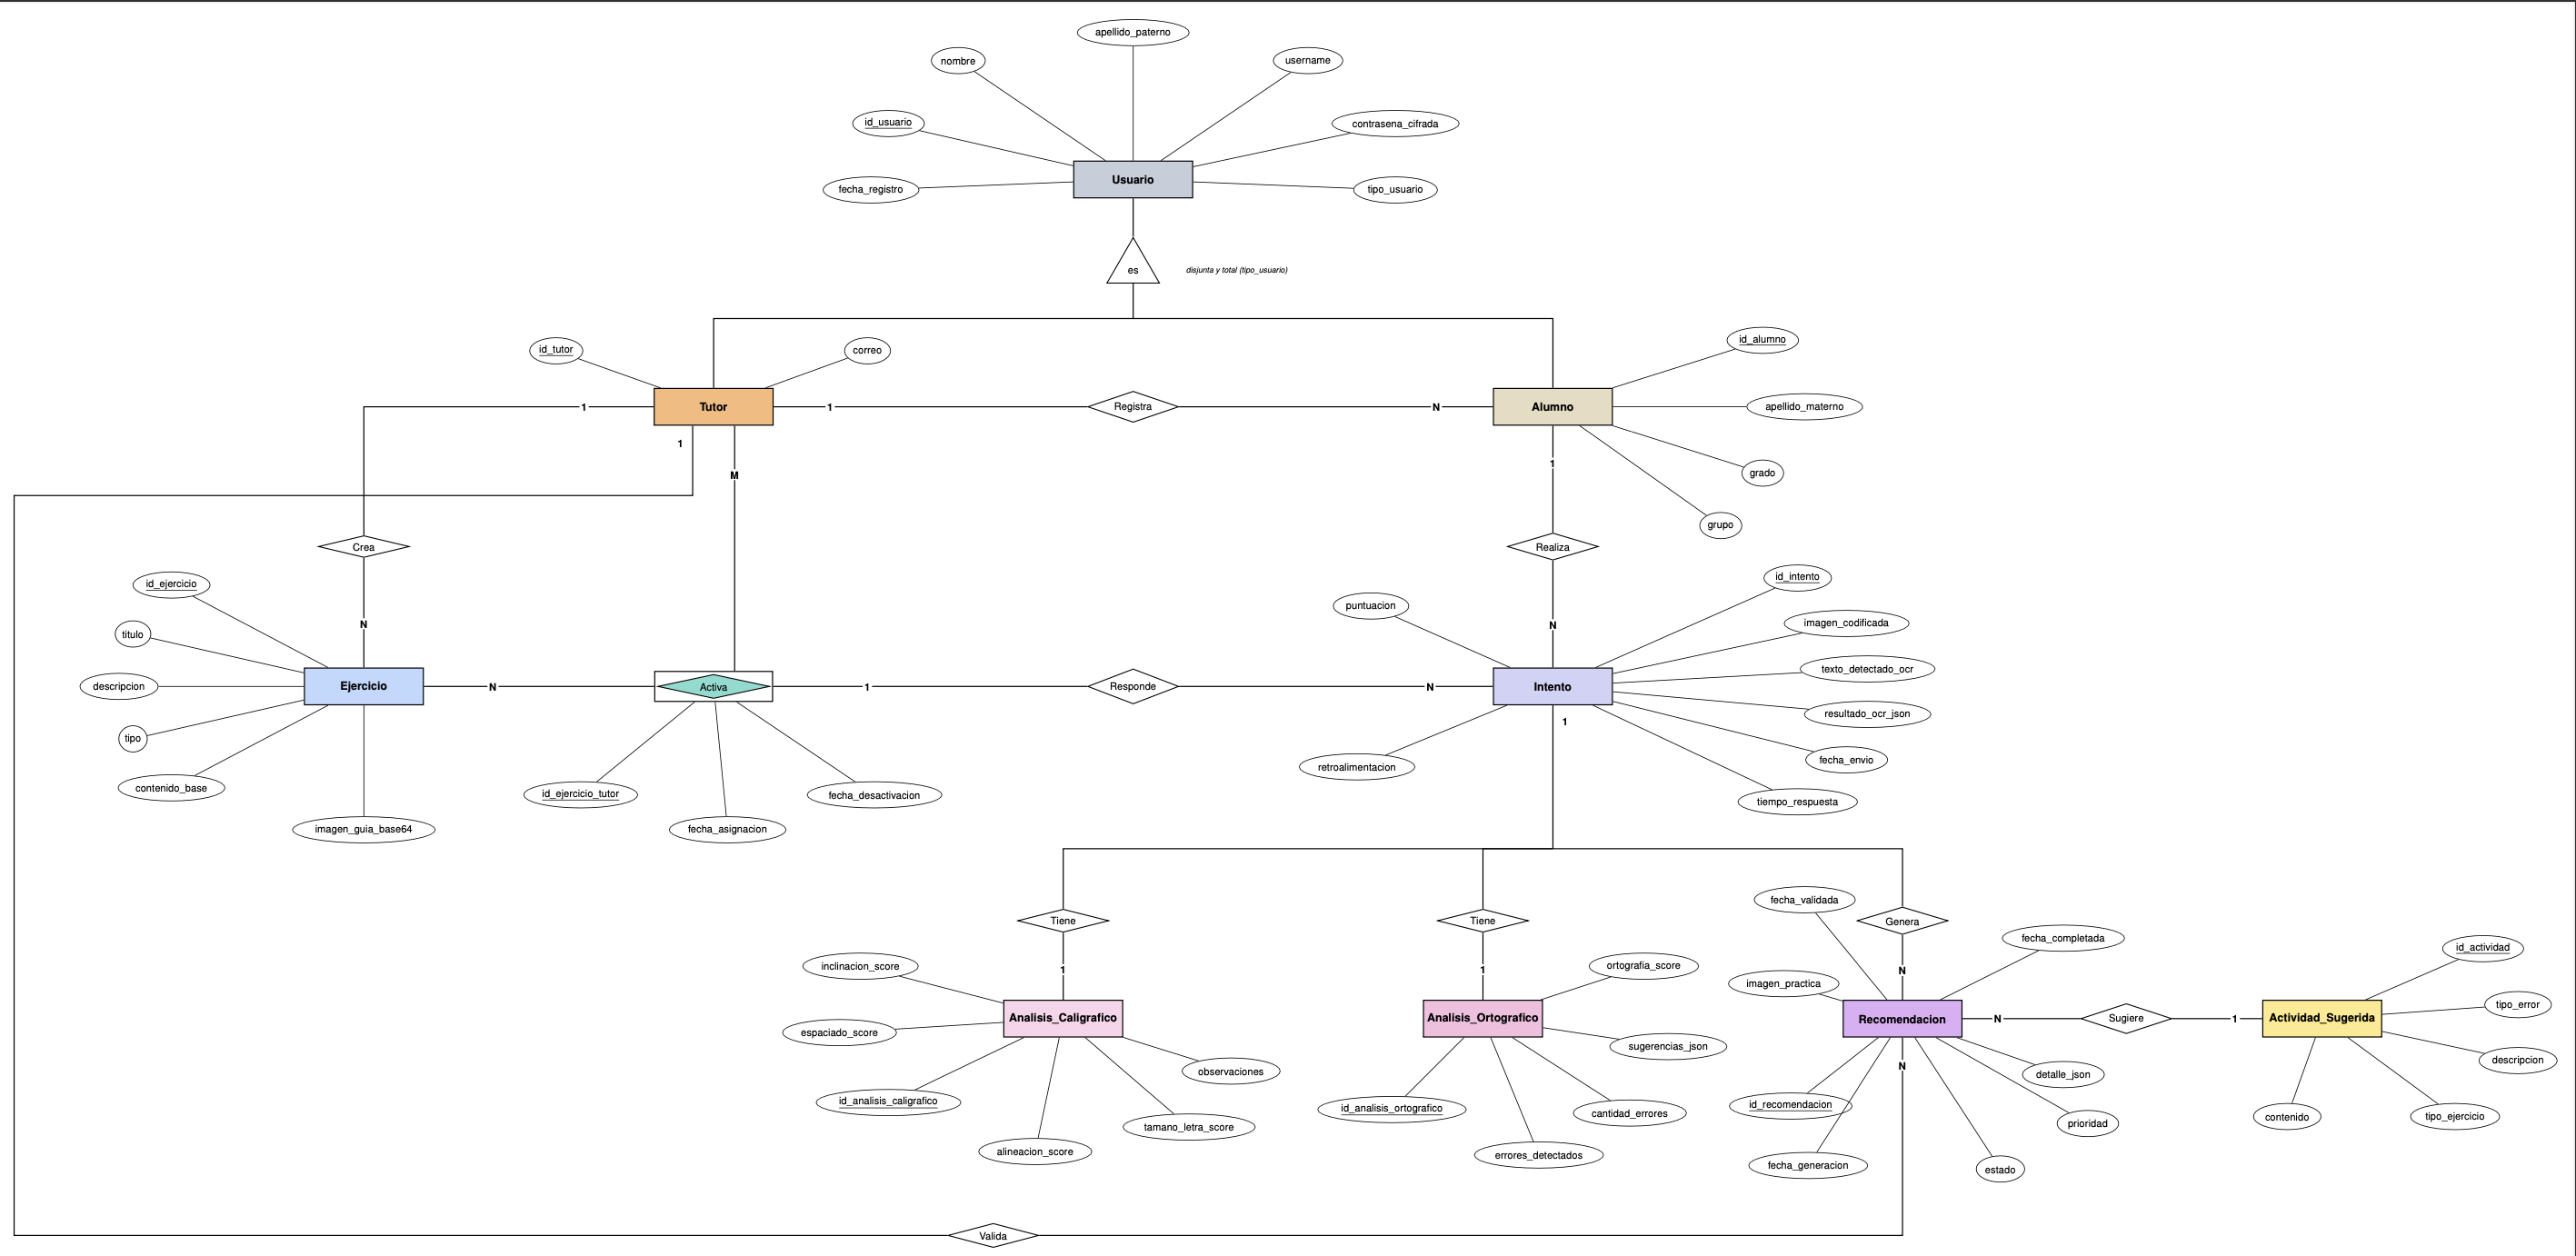
\includegraphics[width=\linewidth,height=0.85\textheight,keepaspectratio]{Imagenes/diagramaER.png}
  \caption{Diagrama entidad relación.}
  \label{fig:er}
\end{figure}
\end{landscape}
  

Cada intento puede carecer de análisis confirmado o tener uno de cada tipo. La restricción única sobre \texttt{id\_intento} en las tablas de análisis impide duplicar resultados del mismo tipo. La revisión posterior actualiza ese registro, mientras la sugerencia original permanece en el JSON del intento. Por tanto, no se modela una evaluación confirmada obligatoria en el momento de la entrega.

\subsubsection{Diccionario de entidades}
\begin{longtable}{p{3.4cm}p{11cm}}
\caption{Entidades de usuarios y asignaciones}\label{tab:entidades_usuarios}\\
\toprule Entidad & Función y atributos principales \\ \midrule
\endfirsthead
\toprule Entidad & Función y atributos principales \\ \midrule
\endhead
Estatus & Catálogo de estados: \texttt{id\_estatus} y \texttt{descripcion}. Permite desactivar registros sin borrar su historial. \\
Usuario & Identidad de acceso: \texttt{id\_usuario}, nombre, apellido paterno, \texttt{username}, hash de contraseña, tipo de usuario, fecha de registro y estado. \\
Tutor & Perfil asociado a un usuario mediante una llave única. Contiene \texttt{id\_tutor}, \texttt{id\_usuario} y correo. \\
Alumno & Perfil del estudiante: \texttt{id\_alumno}, \texttt{id\_usuario}, \texttt{id\_tutor}, apellido materno, grado y grupo. \\
Ejercicios & Catálogo con título, descripción, tipo, \texttt{contenido\_base}, imagen guía opcional, tutor creador opcional y estado. El JSON configura las respuestas aceptadas. \\
Ejercicios\_Tutor & Asignación del catálogo a un tutor: identificadores de ejercicio y tutor, estado, \texttt{fecha\_asignacion} y \texttt{fecha\_desactivacion}. \\
\bottomrule
\end{longtable}

\begin{longtable}{p{3.4cm}p{11cm}}
\caption{Entidades del proceso de evaluación}\label{tab:entidades_evaluacion}\\
\toprule Entidad & Función y atributos principales \\ \midrule
\endfirsthead
\toprule Entidad & Función y atributos principales \\ \midrule
\endhead
Intentos & Entrega con \texttt{id\_intento}, alumno, asignación, \texttt{imagen\_codificada}, \texttt{texto\_detectado\_ocr}, \texttt{resultado\_ocr\_json}, fecha, tiempo de respuesta opcional, puntuación y retroalimentación. \\
Análisis ortográfico & Tabla \texttt{Analisis\_Ortografico}: identificador, intento único, \texttt{ortografia\_score}, \texttt{cantidad\_errores}, \texttt{sugerencias\_json} y campo opcional \texttt{errores\_detectados}. El flujo CLS guarda los conteos y la confirmación dentro del JSON. \\
Análisis caligráfico & Tabla \texttt{Analisis\_Caligrafico}: identificador, intento único, \texttt{alineacion\_score}, \texttt{tamano\_letra\_score}, \texttt{espaciado\_score}, \texttt{inclinacion\_score} y \texttt{observaciones}. \\
\bottomrule
\end{longtable}

\subsubsection{Esquema relacional de la evaluación}
La Figura~\ref{fig:rel} detalla las claves y campos que conectan la entrega con los resultados. PK denota llave primaria, FK llave foránea y UQ una restricción de unicidad. La vista de progreso deriva sus datos de los análisis y no constituye una tabla adicional.


  \begin{landscape}
  \begin{figure}[p]
    \centering
    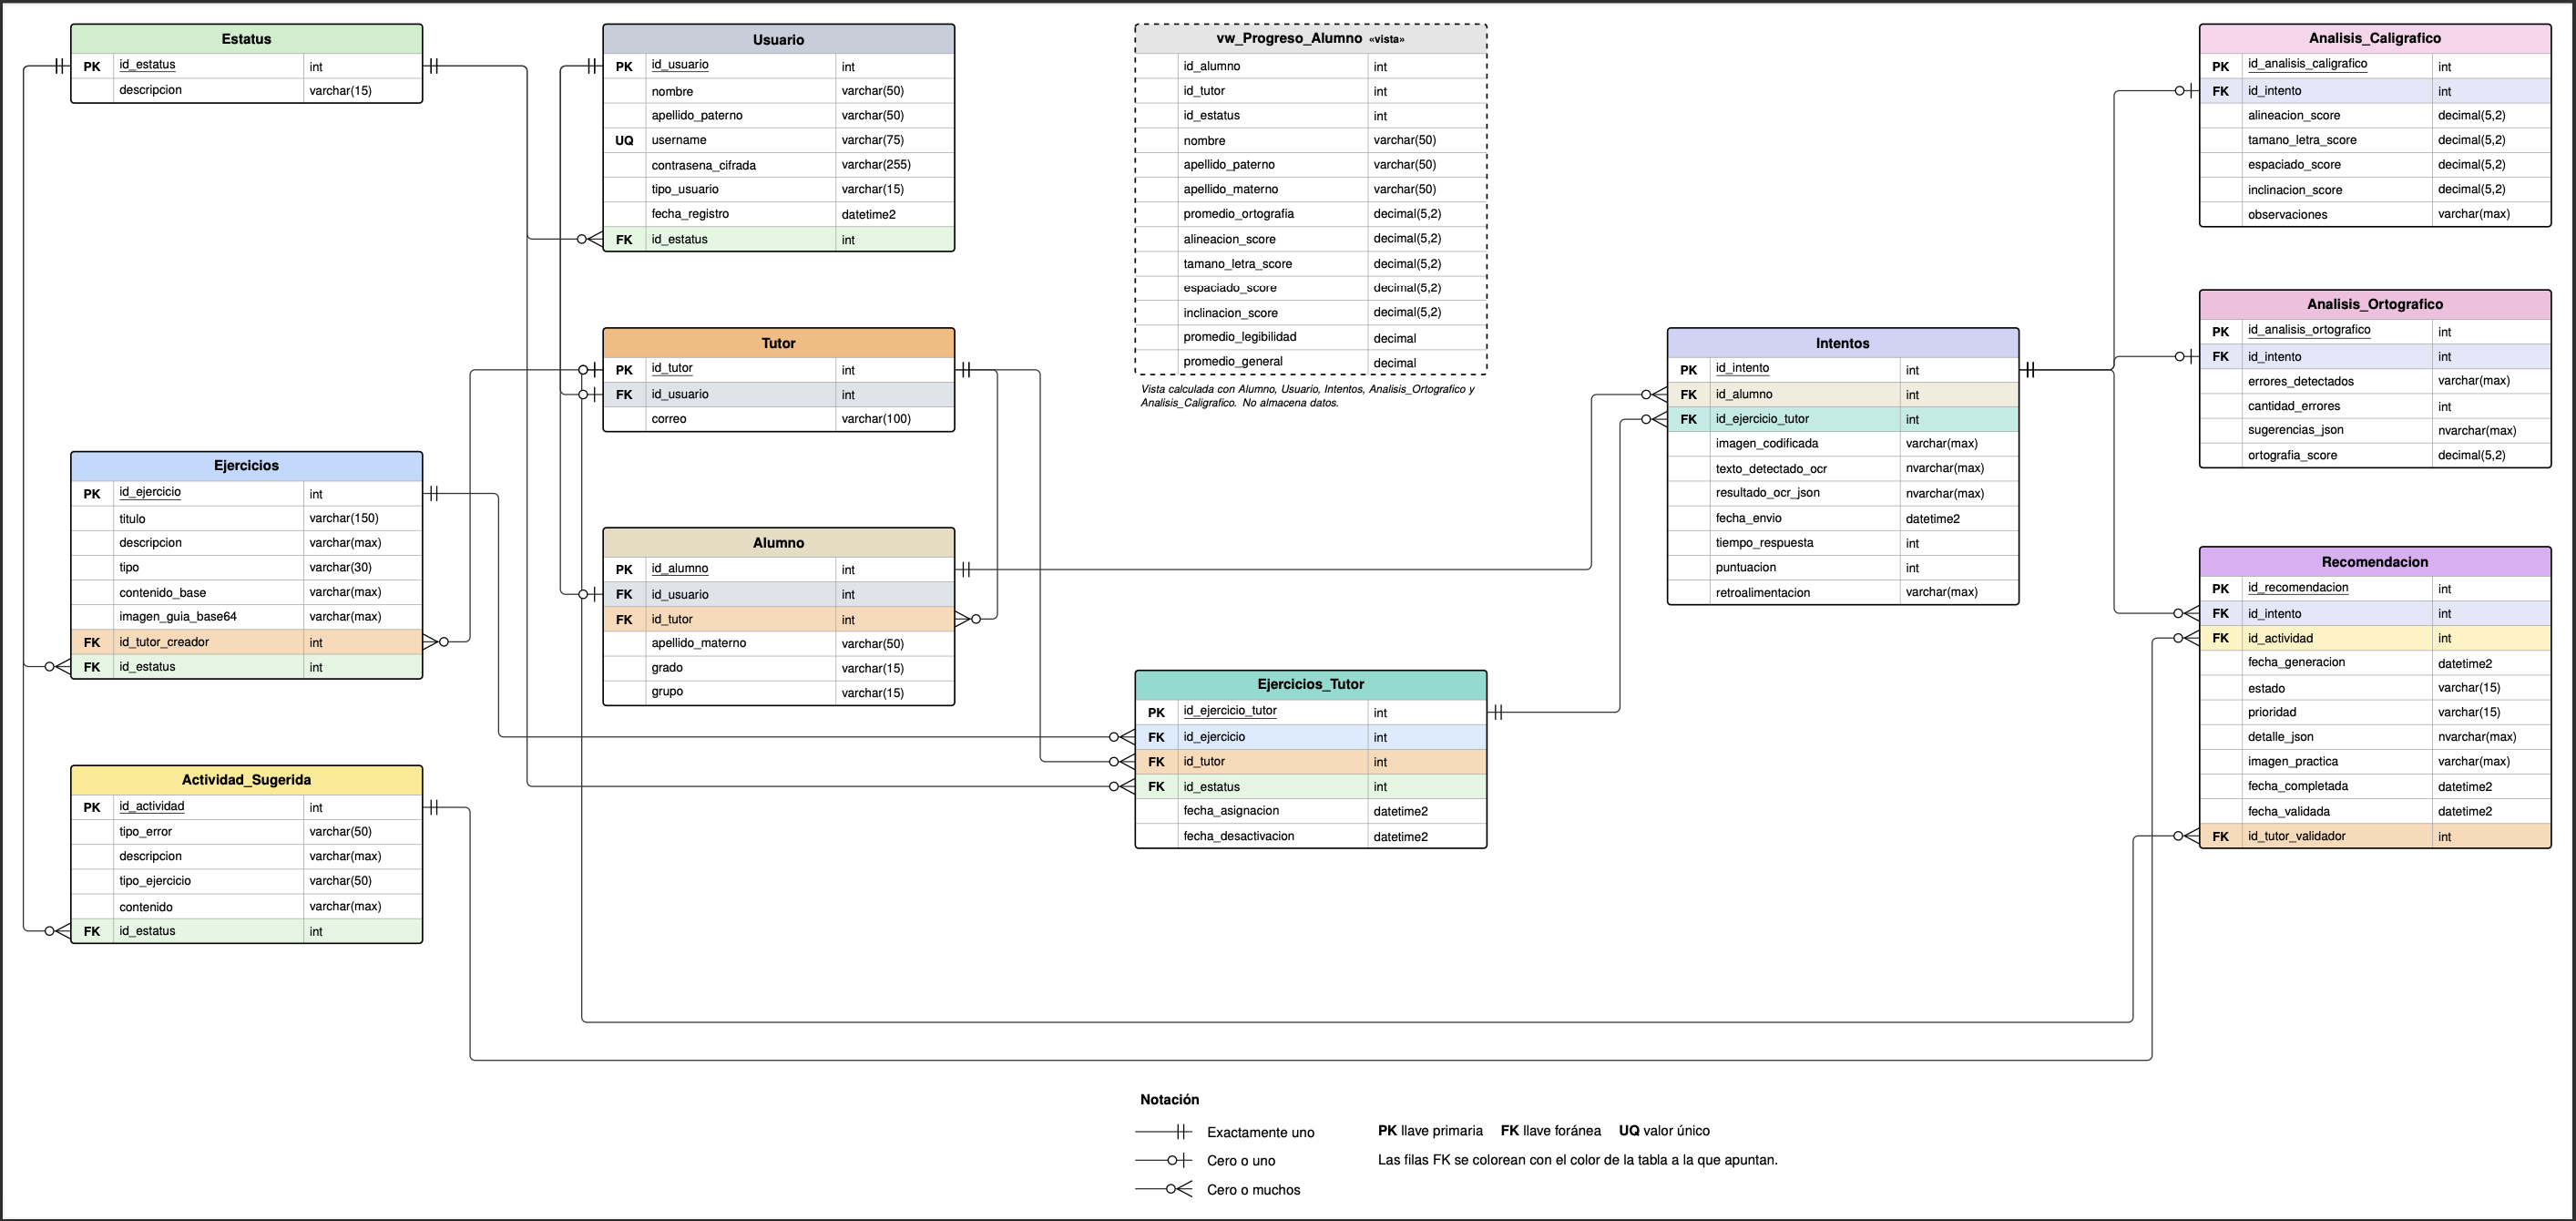
\includegraphics[width=\linewidth,height=0.85\textheight,keepaspectratio]{Imagenes/DiagramaREL.png}
    \caption{Diagrama relacional.}
    \label{fig:rel}
  \end{figure}
  \end{landscape}

\subsubsection{Persistencia, confirmación y trazabilidad}
\texttt{texto\_detectado\_ocr} almacena la transcripción, mientras \texttt{resultado\_ocr\_json} conserva las anotaciones del proveedor y las sugerencias locales. Se distingue así la evidencia automática del resultado confirmado. La revisión guarda la puntuación y retroalimentación del intento y, cuando se proporcionan, los análisis de ortografía y legibilidad dentro de una misma transacción. Una excepción provoca la reversión de esos cambios.

El historial se consulta directamente sobre \texttt{Intentos}, sus ejercicios y sus análisis. La migración \texttt{004\_progreso\_vista.sql} define \texttt{vw\_Progreso\_Alumno} y sustituye las tablas antiguas de promedios e instantáneas. El diseño vigente no utiliza disparadores para sincronizar el progreso ni una vista denominada \texttt{vw\_historial\_alumno}. Corregir un análisis cambia el promedio consultado; no se conserva una versión histórica de cada corrección del tutor.

\subsubsection{Persistencia de las recomendaciones}
\label{sec:bd-recomendaciones}
\begin{table}[H]
\centering
\caption{Estructuras para generar y consultar recomendaciones}\label{tab:entidades_SR}
\begin{tabular}{p{3.8cm}p{10.4cm}}
\toprule Estructura & Responsabilidad \\ \midrule
Vista de progreso & \texttt{vw\_Progreso\_Alumno} proporciona los promedios de ortografía y legibilidad al guardar la calificación. \\
Actividad\_Sugerida & Identifica los tipos de práctica asociados con un promedio bajo de ortografía o legibilidad. \\
Recomendacion & Vincula el intento con un tipo de práctica. Guarda el contenido de la ficha en \texttt{detalle\_json}, el estado y la evidencia de la práctica. \\
\bottomrule
\end{tabular}
\end{table}
La migración \texttt{007\_retroalimentacion.sql} agrega \texttt{detalle\_json}, un índice por intento y los tipos de actividad que utiliza el servicio. El JSON guarda, entre otros datos, el motivo de la recomendación, el promedio consultado, las instrucciones y el modelo que se imprime. Así, el panel del alumno, el detalle del tutor y la descarga recuperan la misma actividad.

Al volver a calificar, la aplicación puede reemplazar o retirar la recomendación según los promedios confirmados. El almacenamiento de evidencias y su validación docente forman parte del seguimiento previsto en el RF-31.
